\documentclass[tikz,border=10pt]{standalone}
\usetikzlibrary{angles,quotes}
\begin{document}
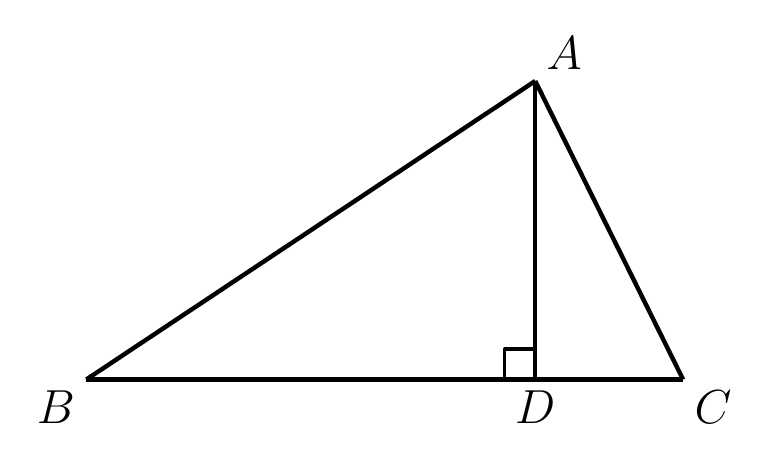
\begin{tikzpicture}[line join=round, line width=1.6pt]
\coordinate (A) at (1.891,1.902);
\coordinate (B) at (-3.810,-1.889);
\coordinate (C) at (3.769,-1.889);
\coordinate (D) at (1.891,-1.889);



\draw (A) -- (B);
\draw (B) -- (C);
\draw (C) -- (A);

\draw (A) -- (D);

\draw (B) -- (D);
\draw (D) -- (C);

\draw pic[draw, angle radius=0.387cm, line width=1.2pt] {right angle=A--D--B};

\node[above right] at (A) {\fontsize{16.5}{19.8}\selectfont $A$};
\node[below left] at (B) {\fontsize{16.5}{19.8}\selectfont $B$};
\node[below right] at (C) {\fontsize{16.5}{19.8}\selectfont $C$};
\node[below] at (D) {\fontsize{16.5}{19.8}\selectfont $D$};
\end{tikzpicture}
\end{document}